\documentclass[xcolor=dvipsnames,aspectratio=169]{beamer}
\usepackage[utf8]{inputenc}
\usetheme{Warsaw}
\usepackage{pgfpages}

% -----------------------------------------------------------------------------
% Notes toggle
% Compile with \def\NOTES{} before \input if you want notes-only output.
% -----------------------------------------------------------------------------
\newif\ifnotes
\ifdefined\NOTES\notestrue\fi
\ifnotes
  \setbeameroption{show only notes}
\else
  \setbeameroption{hide notes}
\fi

% -----------------------------------------------------------------------------
% Shared formatting
% -----------------------------------------------------------------------------
\setcounter{tocdepth}{2}

% =============================================================================
% Theme settings
% =============================================================================

% --- Core theme colors ---
\definecolor{ThemePrimary}{rgb}{0.0745, 0.1608, 0.2941}   % deep blue
\definecolor{ThemeSecondary}{rgb}{0.8667, 0.2039, 0.0118} % warm red/orange
\definecolor{ThemeAccent}{rgb}{0.1137, 0.3451, 0.6549}    % medium blue
\definecolor{ThemeLight}{rgb}{0.9725, 0.9804, 0.9882}     % near white
\definecolor{ThemeText}{rgb}{0.10, 0.10, 0.10}

% --- Optional extra palette ---
\definecolor{ThemeHighlight}{rgb}{0.9608, 0.5294, 0.1176}
\definecolor{ThemeSoftBlue}{rgb}{0.0000, 0.6235, 0.8314}
\definecolor{ThemeSoftNavy}{rgb}{0.1176, 0.2196, 0.4667}

% =============================================================================
% Beamer color settings
% =============================================================================

\setbeamercolor{palette primary}{bg=ThemePrimary,fg=ThemeLight}
\setbeamercolor{structure}{fg=ThemePrimary}
\setbeamercolor{section in toc}{fg=ThemePrimary}
\setbeamercolor{frametitle}{bg=ThemeSecondary,fg=ThemeLight}
\setbeamercolor{frametitle right}{bg=ThemePrimary}
\setbeamercolor{titlelike}{bg=ThemeSecondary,fg=ThemeLight}

% Optional tweaks you can enable later if desired:
% \setbeamercolor{block title}{bg=ThemePrimary,fg=ThemeLight}
% \setbeamercolor{block body}{bg=ThemeLight,fg=ThemeText}
% \setbeamercolor{section in head/foot}{bg=ThemeSoftNavy,fg=ThemeLight}
% \setbeamercolor{subsection in head/foot}{bg=ThemePrimary,fg=ThemeLight}

% =============================================================================
% Footline with page numbers
% =============================================================================

\defbeamertemplate*{footline}{shadow theme}{
    \leavevmode
    \hbox{%
        \begin{beamercolorbox}[
            wd=.5\paperwidth,
            ht=2.5ex,
            dp=1.125ex,
            leftskip=.3cm plus1fil,
            rightskip=.3cm
        ]{author in head/foot}
            \usebeamerfont{author in head/foot}\hfill\insertshortauthor
        \end{beamercolorbox}%
        \hskip0pt%
        \begin{beamercolorbox}[
            wd=.5\paperwidth,
            ht=2.5ex,
            dp=1.125ex,
            leftskip=.3cm,
            rightskip=.3cm plus1fil
        ]{title in head/foot}
            \usebeamerfont{title in head/foot}%
            \insertshorttitle\hfill\insertframenumber\,/\,\inserttotalframenumber
        \end{beamercolorbox}%
    }
    \vskip0pt
}

% =============================================================================
% Headline with current section / subsection
% =============================================================================

\setbeamertemplate{headline}{%
  \leavevmode
  \hbox{%
    \begin{beamercolorbox}[
        wd=.5\paperwidth,
        ht=2.1ex,
        dp=0.7ex,
        leftskip=0.3cm
    ]{section in head/foot}
      \usebeamerfont{section in head/foot}\insertsectionhead
    \end{beamercolorbox}%
    \begin{beamercolorbox}[
        wd=.5\paperwidth,
        ht=2.1ex,
        dp=0.7ex,
        rightskip=0.3cm
    ]{subsection in head/foot}
      \usebeamerfont{subsection in head/foot}\hfill\insertsubsectionhead
    \end{beamercolorbox}%
  }%
}

% =============================================================================
% Automatic outline slides
% =============================================================================

\AtBeginSection[]{
    \begin{frame}{Outline}
        \tableofcontents[currentsection]
    \end{frame}
}

\AtBeginSubsection[]{
    \begin{frame}{Outline}
        \tableofcontents[currentsection,currentsubsection]
    \end{frame}
}

% =============================================================================
% Figure / table packages
% =============================================================================

\usepackage{graphicx}   % figures
\usepackage{float}      % figure/table placement
\usepackage{rotating}   % rotated figures/tables
\usepackage{caption}    % captions
\usepackage{subcaption} % subfigures
\usepackage{makecell}   % table formatting
\usepackage{longtable}  % multipage tables
\usepackage{array}      % custom columns
\usepackage{tabularx}   % flexible-width tables
\usepackage{booktabs}   % professional tables

\newcolumntype{L}{>{\raggedright\arraybackslash}m{4cm}}
\newcolumntype{R}[1]{>{\raggedright\arraybackslash\hspace{0pt}\vspace{-0.25cm}}p{#1}}

% =============================================================================
% Math packages
% =============================================================================

\usepackage{amsfonts}
\usepackage{mathrsfs}
\usepackage{amsmath}
\usepackage{amssymb}
\usepackage{amsthm}
\usepackage{mathtools}
\usepackage{steinmetz}

% =============================================================================
% Chemistry / units
% =============================================================================

\usepackage[version=4]{mhchem}
\usepackage{chemformula}

\usepackage{siunitx}
\sisetup{locale = DE}
\sisetup{output-decimal-marker = {.}}

% =============================================================================
% Code / URL / verbatim
% =============================================================================

\usepackage{listings}
\usepackage{url}
\usepackage{verbatim}

% =============================================================================
% End of format file
% =============================================================================


% -----------------------------------------------------------------------------
% Presentation metadata
% Update these for each new talk.
% -----------------------------------------------------------------------------
\newcommand{\TalkTitle}{State-Space Models}
\newcommand{\TalkAuthor}{Soo Min Kimm}
\newcommand{\TalkInstitute}{}
\newcommand{\TalkDate}{21/10/25}

\title{\TalkTitle}
\author{\TalkAuthor}
\institute{\TalkInstitute}
\date{\TalkDate}

\begin{document}
    \begin{frame}
        \titlepage
    \end{frame}
    
    \begin{frame}{Outline}
        \tableofcontents
    \end{frame}

    \section{Background}
        \subsection{Linear Time-Invariant (LTI) System}
            \begin{frame}{LTI System}
                \begin{block}{Linearity}
                    If the system's input-output relationship is $u(t) \mapsto y(t)$, then for any two inputs $u_{1} (t)$ and $u_{2} (t)$ and scalars $\alpha, \beta$, 
                    $$\text{If } y_1(t) = \mathcal{T}[u_1(t)] \text{ and } y_2(t) = \mathcal{T}[u_2(t)], \text{ then }\mathcal{T}[\alpha u_1(t) + \beta u_2(t)] = \alpha y_1(t) + \beta y_2(t)$$
                \end{block}

                \begin{block}{Time-Invariance}
                    If the input is shifted in time by $\tau$, then the output is shifted by the same $\tau$,
                    $$\mathcal{T}[u(t - \tau)] = y(t - \tau)$$
                \end{block}
            \end{frame}

            \begin{frame}{Connection to Convolution}
                \small
                Denote the system as an operator $\mathcal{T}$ that maps an input signal $u(t)$ to an output signal $y(t)$, i.e., $y(t) = \mathcal{T}[u(t)]$. \\
                Suppose an input is an impulse $u(t) = \delta(t)$, then the output $y(t) \ = h(t)$ is an impulse response. \\
                Any input $u(t)$ can be decomposed as $u(t) = \int_{\tau} u(\tau) \delta (t - \tau) \; d\tau$. \\
                If the system is linear, $\mathcal{T}[u(t)] = \int_{\tau} u(\tau)\, \mathcal{T}[\delta(t - \tau)]$. \\
                If the system is time-invariant, $\mathcal{T}[\delta(t - \tau)] = h(t - \tau)$. \\
                Hence, for the LTI system, 
                $$y(t) = \mathcal{T}[u(t)] = \int_{\tau} u(\tau) h(t - \tau) = (h * u)(t)$$
                In the frequency domain, the convolution becomes multiplication 
                $$Y(\omega) = H(\omega) U(\omega)$$ 
                where $H(\omega)$ is a transfer function.
            \end{frame}

        \subsection{Projection}
            \begin{frame}{Intuition}
                \begin{figure}
                    \centering
                    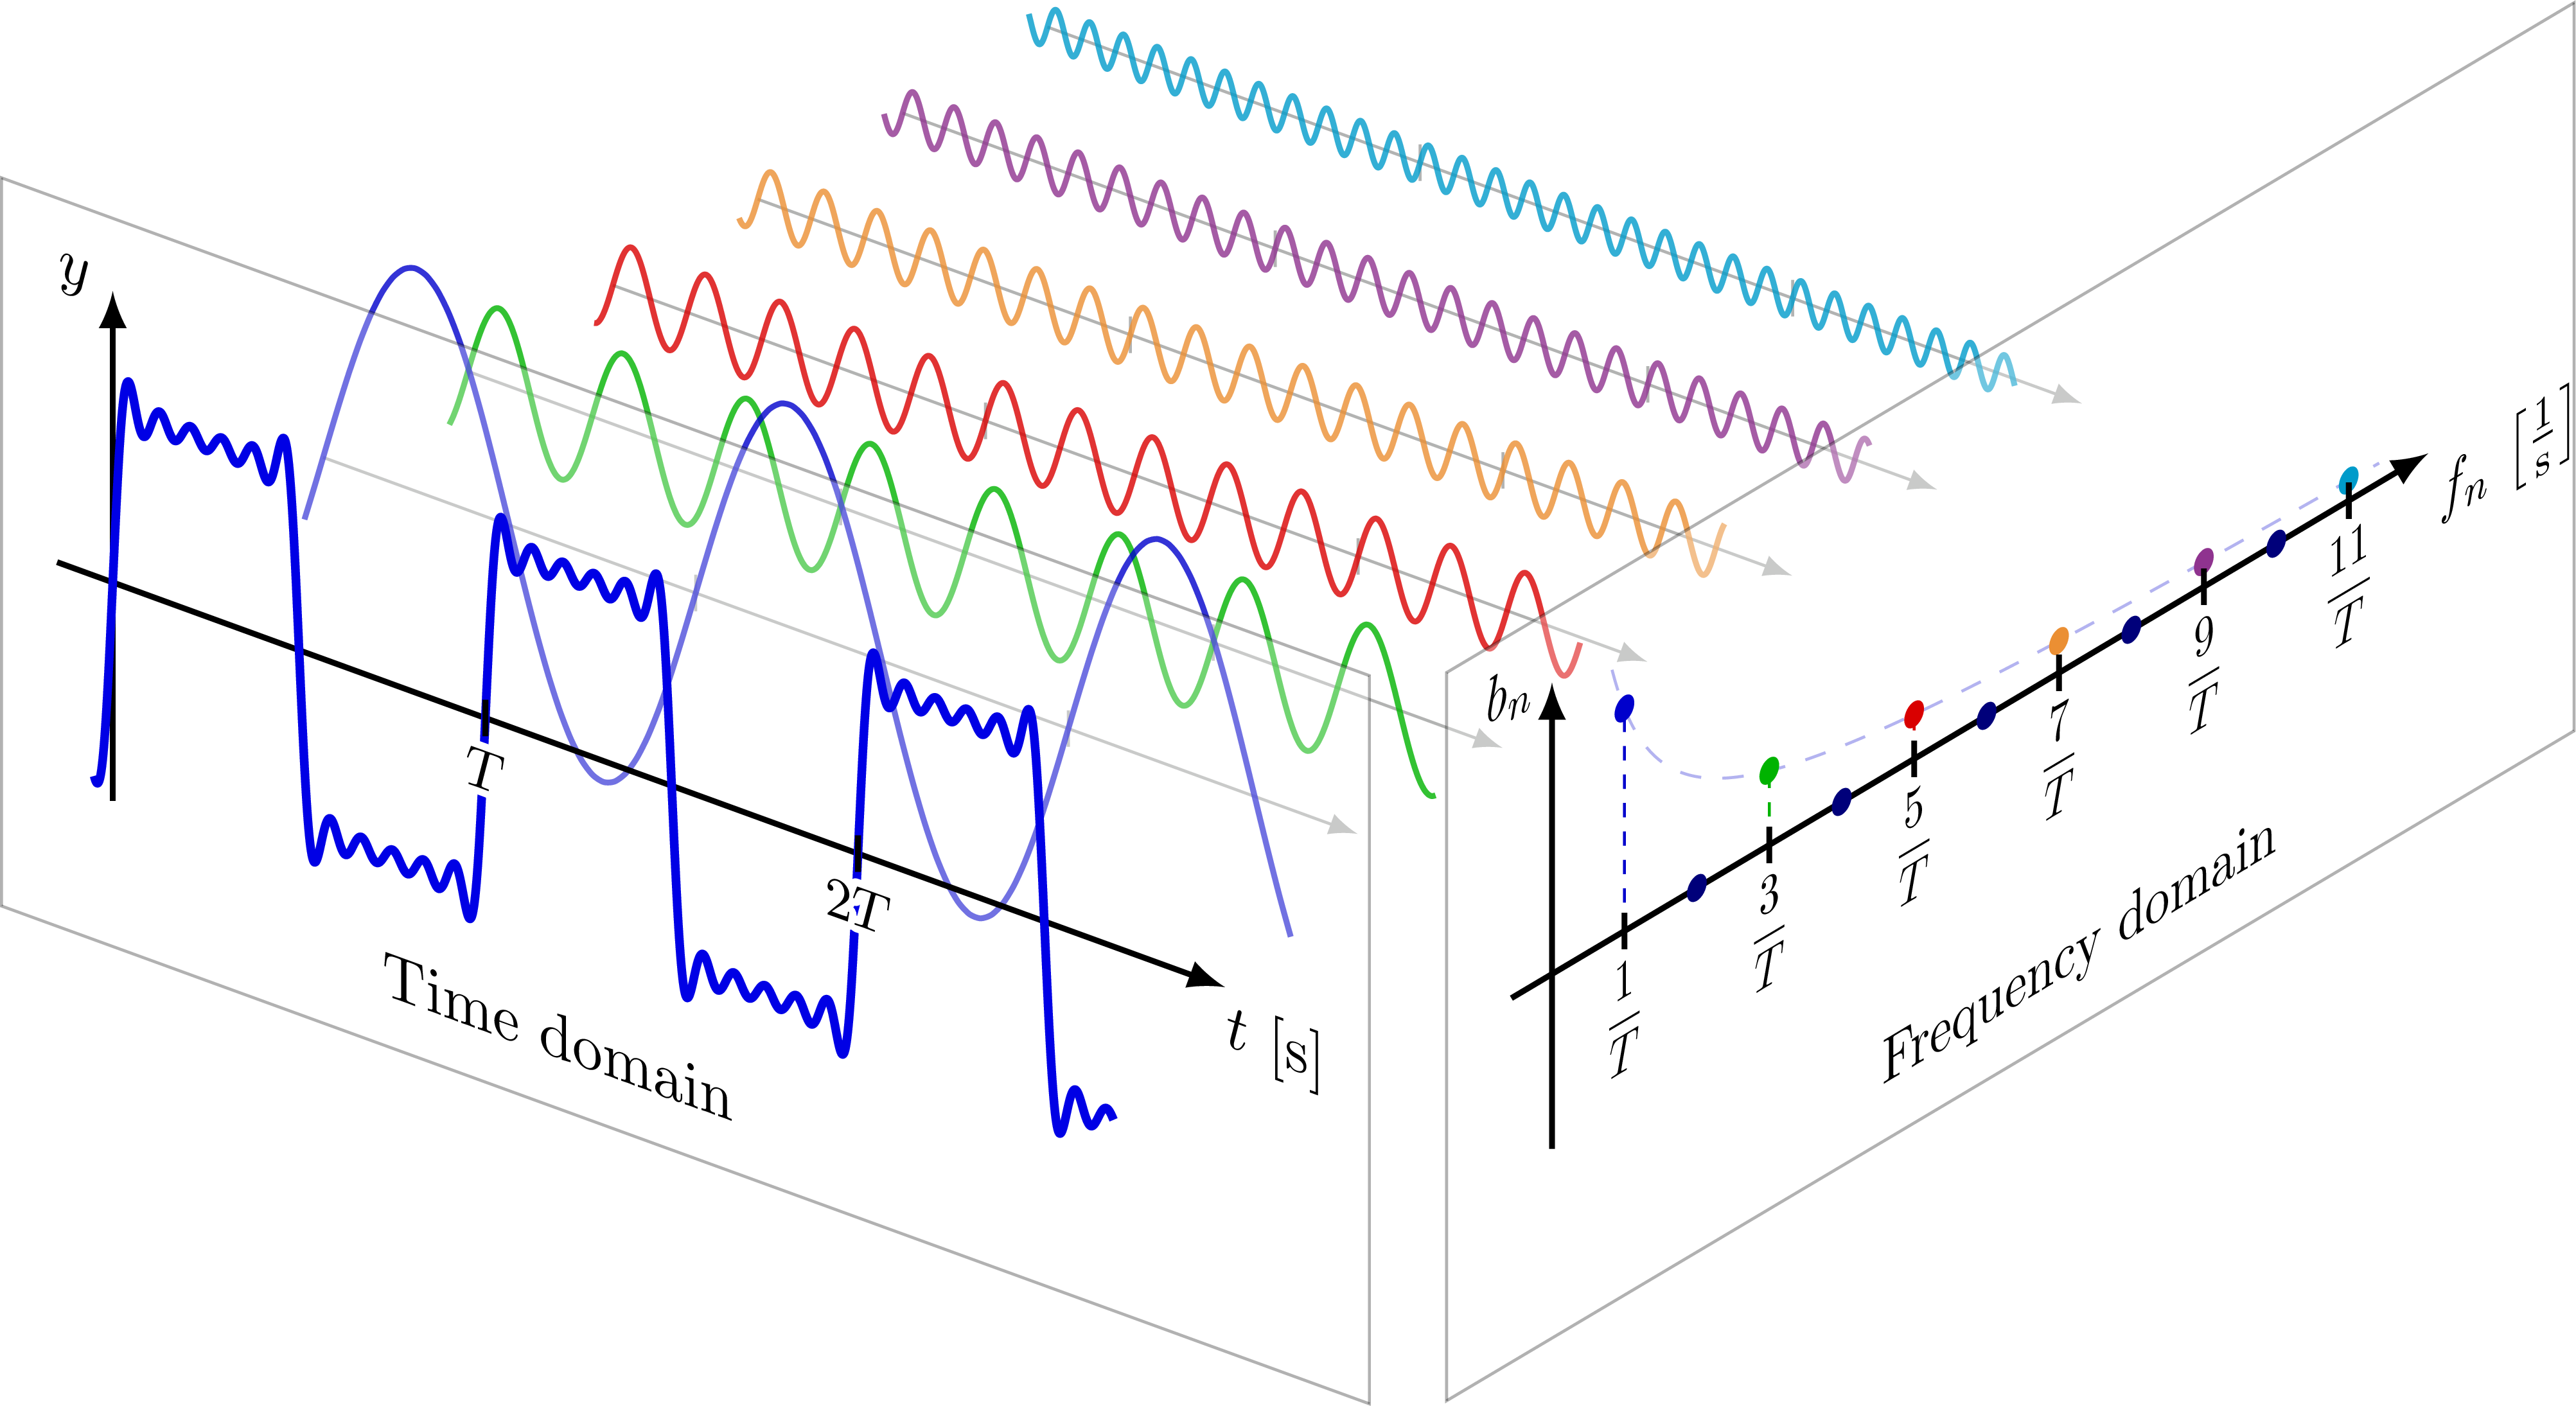
\includegraphics[width=0.7\linewidth]{figure/fourier_transform.png}
                    \caption{Fourier transform. Image from \url{https://dibsmethodsmeetings.github.io/fourier-transforms/}}
                    \label{fig:fourier_transform}
                \end{figure}
            \end{frame}
        
            \begin{frame}{Basis Function}
                In function spaces, a set of functions $\{ \phi_{0} (x), \phi_{1} (x), \cdots \}$ are basis functions if a function $f(x)$ can be approximated as a linear combination $f(x) \approx \sum_{n = 0}^{N} c_{n} \phi_{n} (x)$ where $c_{n}$ is a projection coefficient.
                Basis functions must be linearly independent.
            \end{frame}

            \begin{frame}{Orthogonality}
                If an inner product is defined as
                $$\langle f, g \rangle = \int f(x) g(x) w(x) \; dx$$
                where $w(x)$ is the weight function, then orthogonal basis functions satisfy
                $$\langle \phi_{m}, \phi_{n} \rangle = 0 \text{ if } m \neq n$$
                Projection coefficient is given by $c_{n} = \frac{\langle f, \phi_{n} \rangle}{\langle \phi_{n}, \phi_{n} \rangle}$.
            \end{frame}

            \begin{frame}{Legendre Polynomials}
                Legendre polynomials $\{ P_{n} (x) \}_{n = 0}^{\infty}$ are defined on the interval $[-1, 1]$ as the solutions to Legendre's differential equation
                $$\frac{d}{dx} [(1 - x^{2}) \frac{d}{dx}P_{n} (x) ] + n(n + 1) P_{n} (x) = 0$$ \\
                A direct definition is 
                $$P_{n} (x) = \frac{1}{2^{n} n!} \frac{d^{n}}{dx^{n}} [(x^{2} - 1)^{n}]$$
                Legendre polynomials are orthogonal on $[-1, 1]$ w.r.t. the weight function $w(x) = 1$. \\

                \begin{itemize}
                    \item $(1 - x^{2}) P_{n}^{\prime} (x) = -nx P_{n} (x) + n P_{n - 1} (x)$
                    \item $(n + 1) P_{n + 1} (x) = (2n + 1)x P_{n} (x) - n P_{n - 1} (x)$
                \end{itemize}
            \end{frame}

        \subsection{Discretisation}
            \begin{frame}{Discretisation}
                \small
                $\frac{d}{dt} x(t) = A x(t) + B u(t)$ can be discretised in the form of $x_{k + 1} = \bar{A} x_{k} + \bar{B} u_{k}$

                \begin{block}{Forward Euler (First-Order Approximation)} 
                    $$\frac{x_{k + 1} - x_{k}}{\Delta} \approx A x_{k} + B u_{k} \Rightarrow x_{k + 1} = (I + \Delta A) x_{k} + \Delta B u_{k}$$
                \end{block}

                \begin{block}{Backward Euler (First-Order Approximation)}
                    $$\frac{x_{k + 1} - x_{k}}{\Delta} \approx A x_{k + 1} + B u_{k + 1} \Rightarrow x_{k + 1} = (I - \Delta A)^{-1} x_{k} + (I - \Delta A)^{-1} \Delta B u_{k + 1}$$
                \end{block}

                \begin{block}{Bilinear Transform (Second-Order Approximation)} 
                    $$\frac{x_{k + 1} - x_{k}}{\Delta} \approx \frac{1}{2} (A x_{k} + A x_{k + 1} + B u_{k} + B u_{k + 1})$$
                    $$\Rightarrow x_{k+1} = (I - \frac{\Delta}{2} A)^{-1}(I + \frac{\Delta}{2} A) x_{k} + (I - \frac{\Delta}{2} A)^{-1} \frac{\Delta}{2} B (u_{k} + u_{k + 1})$$
                \end{block}
            \end{frame}

            \begin{frame}{Discretisation}
                \begin{block}{Zero-Order Hold (ZOH)}
                    For any interval, the exact solution to ODE is given by 
                    $$x(t) = e^{A (t - t_{0})} x(t_{0}) + \int_{s = t_{0}}^{t} e^{A(t - s)} B u(s) \; ds$$
                    Assume $u(s) = u_{k}$ is piecewise constant on each interval $s \in [k \Delta, (k + 1) \Delta]$ for a learned step size $\Delta$. \\
                    Set $t_{0} = k \Delta$, $t = (k + 1) \Delta$, and $\tau = t - s$, then 
                    $$x_{k + 1} = e^{A \Delta} x_{k} + (\int_{\tau = 0}^{\Delta} e^{A \tau} d \tau) B u_{k}$$
                    If $A$ is invertible, then $\frac{d}{d \tau} (e^{A \tau}) = A e^{A \tau} \iff e^{A \tau} = A^{-1} \frac{d}{d \tau} e^{A \tau}$ and $\int_{\tau = 0}^{\Delta} e^{A \tau} d \tau = A^{-1} [e^{A \tau}]_{\tau=0}^{\Delta} = A^{-1} (e^{A \Delta} - I)$.
                \end{block}
            \end{frame}

        \subsection{Properties of Matrices}
            \begin{frame}{Definition}
                \begin{block}{Symmetry}
                    $A \in \mathbb{R}^{N \times N}$ is symmetric if $A^{T} = A$.
                \end{block}
            
                \begin{block}{Normality}
                    $A \in \mathbb{C}^{N \times N}$ is normal if $A^{*}A = AA^{*}$.
                \end{block}

                \begin{block}{Orthogonality}
                    $V \in \mathbb{R}^{N \times N}$ is orthogonal if $V^{T}V = I \iff V^{-1} = V^{T}$.
                \end{block}

                \begin{block}{Unitarity}
                    $U \in \mathbb{C}^{N \times N}$ is unitary if $U^{*}U = I \iff U^{-1} = U^{*}$.
                \end{block}
            \end{frame}

            \begin{frame}{Definition}
                \begin{block}{Diagonality}
                    $A$ is orthogonally diagonalisable if $A$ is similar to a diagonal matrix $D$ w/ an orthogonal matrix $V$, i.e. $A = VDV^{T}$. \\
                    $A$ is unitarily diagonalisable if $A$ is similar to a diagonal matrix $D$ w/ an unitary matrix $U$, i.e. $A = UDU^{*}$.
                \end{block} 

                \begin{block}{Singular Value}
                    $\forall A \in \mathbb{C}^{M \times N}$, singular values are defined as $\sigma_{i} (A) = \sqrt{\lambda_{i} (A^{*} A)} \geq 0$.
                \end{block}

                \begin{block}{Spectral Norm}
                    $\Vert A \Vert_{2} = \sigma_{max} (A)$, i.e., the largest singular value tells the maximum amplification $A$ can apply to any unit vector.
                \end{block}
            \end{frame}

            \begin{frame}{Theorem}
                \begin{block}{Theorem 1}
                    $A \in \mathbb{R}^{N \times N}$ is symmetric. $\iff A$ is orthogonally diagonalisable.
                \end{block}

                \begin{block}{Theorem 2}
                    $A \in \mathbb{C}^{N \times N}$ is normal. $\iff A$ is unitarily diagonalisable.
                \end{block}

                \begin{block}{Woodbury Matrix Identity}
                    $(A + UCV)^{-1} = A^{-1} + A^{-1} U (C^{-1} + VA^{-1}U)^{-1} VA^{-1}$ where $A \in \mathbb{C}^{N \times N}$, $U \in \mathbb{C}^{N \times k}$, $C \in \mathbb{C}^{k \times k}$, $V \in \mathbb{C}^{k \times N}$. 
                \end{block}
            \end{frame}

            \begin{frame}{Mode \& Coupling}
                \small
                If $A$ is diagonalisable, then $A = V \Lambda V^{-1}$ where $\Lambda = \mathrm{diag} (\lambda_{1}, \cdots, \lambda_{N})$ and $V = [v_{1} \cdots v_{N}]$ \\
                Each pair $(\lambda_{i}, v_{i})$ defines a mode:

                \begin{itemize}
                    \item Decay rate
                    \begin{itemize}
                        \item $\Re (\lambda_{i}) < 0$: Decaying mode $\to$ Memory fades exponentially
                        \item $\Re (\lambda_{i}) = 0$: Persistent mode $\to$ Infinite memory (Oscillation)
                        \item $\Re (\lambda_{i}) > 0$: Growing mode $\to$ Unstable (Exploding memory)
                    \end{itemize}
                    \item Oscillation
                    \begin{itemize}
                        \item $\Im (\lambda_{i}) = 0$: No oscillation
                        \item $\Im (\lambda_{i}) \neq 0$: Sinusoidal oscillation
                    \end{itemize}
                \end{itemize}

                Each eigenvector defines a mode direction, and its eigenvalue dictates how that mode evolves. \\
                Also, $e^{At} = V e^{\Lambda t} V^{-1} = V \mathrm{diag} (e^{\lambda_{i}t}) |_{i = 1}^{n} V^{-1}$. \\
                Coupling is modes influencing each other's evolution:

                \begin{itemize}
                    \item Diagonal: None
                    \item Diagonal + Low-rank: Light global coupling
                    \item Triangular / Dense: Strong hierarchical coupling
                \end{itemize}
            \end{frame}

            \begin{frame}{Transient Amplification}
                Given a homogeneous linear ODE $\frac{d}{dt} x(t) = A x(t)$ w/ solution $x(t) = e^{At} x(0)$, if all eigenvalues of $A$ have negative real parts, then asymptotically $x(t) \to 0$. \\
                When $A$ is normal, the eigenvectors form an orthogonal unitary basis, and energy evolves independently in each mode \\
                When $A$ is non-normal, the directions overlap — energy in one mode can project onto another, causing transient amplification, i.e., $\Vert x(t) \Vert_{2}$ increases before decaying. \\
                The amplification (gain) at time $t$ is $G(t) = \frac{\Vert x(t) \Vert}{\Vert x(0) \Vert}$. \\
                The worst-case amplification is given by $G_{\max} (t) = \underset{t \geq 0}{\sup} \Vert e^{At} \Vert_{2}$.

                \begin{itemize}
                    \item $G_{\max} > 1 \iff A$ is non-normal.
                    \item $G_{\max} = 1 \iff A$ is normal w/ all $\Re(\lambda_{i}) \leq 0$.
                \end{itemize}
            \end{frame}

    \section{State-Space Models (SSM)}
        \subsection{State-Space System}
            \begin{frame}{State-Space System}
                \begin{figure}
                    \centering
                    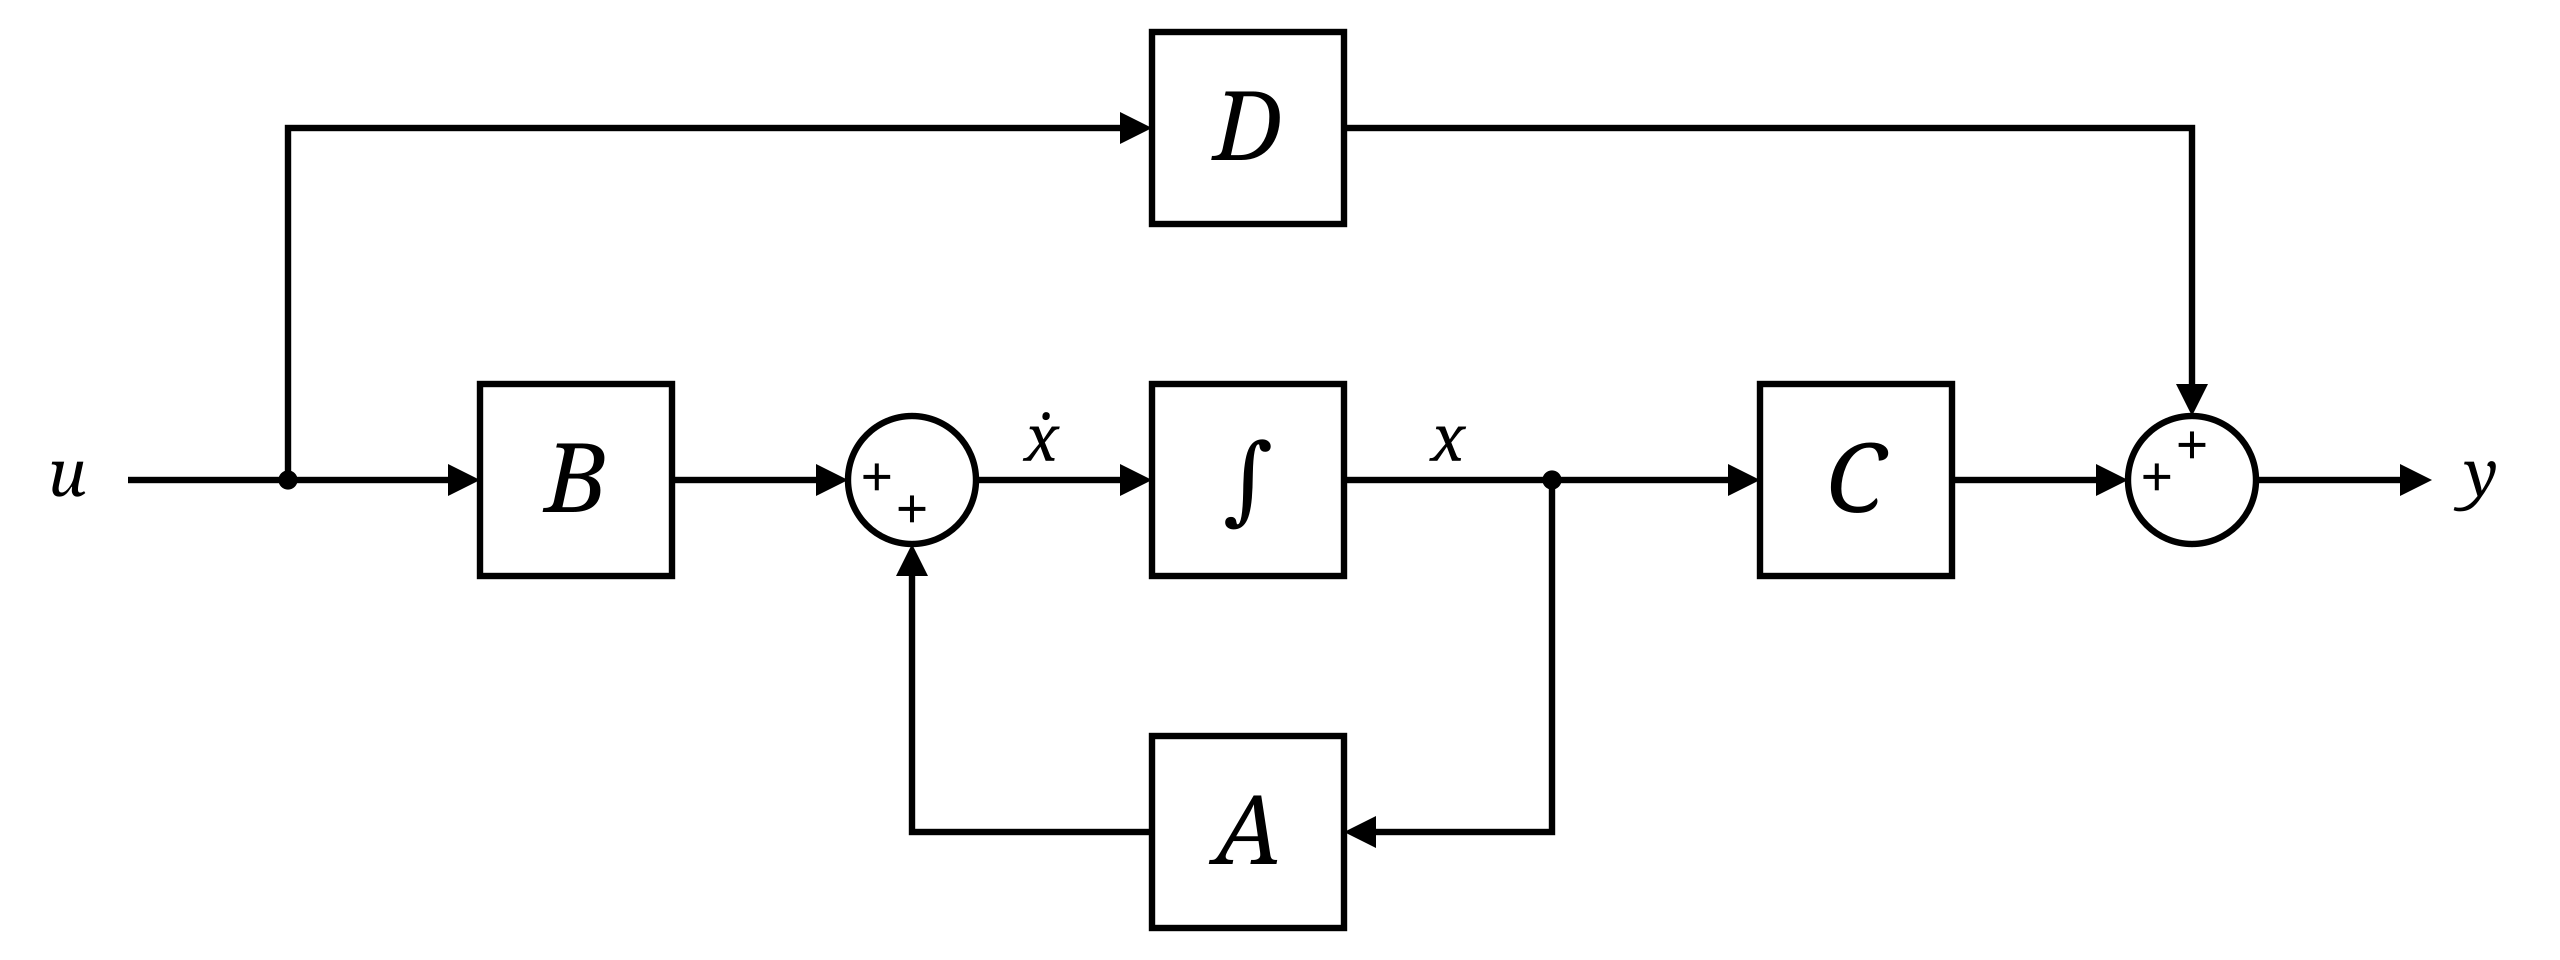
\includegraphics[width=0.7\linewidth]{figure/ssm.png}
                    \caption{SSM. Image from \url{https://www.wikipedia.com/en/articles/State-space_representation}}
                    \label{fig:ssm}
                \end{figure}
            \end{frame}

            \begin{frame}{Continuous-Time Linear State-Space System}
                The system is represented as
                
                \begin{equation*} 
                    \begin{cases}
                        \frac{d}{dt} x(t) = Ax(t) + Bu(t) \\
                        y(t) = C x(t) + D u(t)
                    \end{cases}
                \end{equation*}

                where 

                \begin{itemize}
                    \item $x(t)$: State vector (Hidden memory of the system)
                    \item $u(t)$: Input signal (External sequence coming in)
                    \item $y(t)$: Output signal (Observed sequence)
                    \item $A, B, C, D$: Matrices
                \end{itemize}
                
                Feed-through part $Du(t)$ is the residual connection and can be omitted for the simplicity of the future computation. \\
                The system is LTI iff there are no non-linear functions, and when $A, B, C, D$ are constant matrices which do not depend on $t$. 
            \end{frame}

            \begin{frame}{Discrete-Time Linear State-Space System}
                After discretisation, the system turns into 
                
                \begin{equation*} 
                    \begin{cases}
                        x_{t + 1} = \bar{A} x_{t} + \bar{B} u_{t} \\
                        y_{t} = \bar{C} x_{t} + \bar{D} u_{t}
                    \end{cases}
                \end{equation*}

                where the first equation is the recurrent network. \\
                Unrolling the recurrence, given the entire input history $\{ u_{0}, \cdots, u_{t} \}$, $x_{t} = \bar{A}^{t} x_{0} + \sum_{k = 0}^{t - 1} \bar{A}^{k} \bar{B} u_{t - 1 - k}$ where the first term is the homogeneous term which depends on the initial state, and the second term is the particular solution that represents the convolution w/ past inputs. \\
                Setting $x_{0} = 0$, $y_{t} = \bar{C} (\sum_{k = 0}^{t - 1} \bar{A}^{k} \bar{B} u_{t - 1 - k}) = \sum_{k = 0}^{t - 1} K_{k} u_{t - 1 - k}$ where $K_{k} = \bar{C} \bar{A}^{k} \bar{B}$ is the kernel.
            \end{frame}

        \subsection{High-Order Polynomial Projection Operator (HiPPO)}
            \begin{frame}{HiPPO: Polynomial Projection of History}
                Suppose the past input function is $u(\tau)$ for $\tau \in [0, t]$. \\
                HiPPO approximates the function using a set of basis functions $p_{n} (\cdot)$: 
                $$u(\tau) \approx \sum_{n=0}^{N-1} x_n(t) \, p_n (\frac{\tau}{t})$$
                where $p_{n} (\cdot)$ are orthogonal polynomials and $x_{n} (t)$ are projection coefficients. \\
                $x(t)$ is the memory state — the best degree-$(N - 1)$ polynomial approximation of the full history up to time $t$. \\
                Coefficients are defined by the projection 
                $$x_n(t) = \int_0^t p_n (\frac{\tau}{t}) u(\tau) w_t(\tau) \; d\tau $$
            \end{frame}

            \begin{frame}{HiPPO: Dynamics via Expanding Integration Window}
                Suppose time increases slightly from $t \to t + \Delta t$, then
                
                \begin{enumerate}
                    \item The integration window expands w/ new data $u(t + \Delta t)$
                    \item The basis changes from $p_{n} (\frac{\tau}{t}) \to p_{n} (\frac{\tau}{t + \Delta t})$
                \end{enumerate}

                This adjustment defines a DE for $x(t)$. \\
                Leibniz rule says 
                $$\frac{d}{dt} \int_0^t f(\tau,t) \; d\tau = f(t,t) + \int_0^t \frac{\partial f}{\partial t}(\tau,t) \; d\tau$$
                Let $f(\tau, t) = p_n (\frac{\tau}{t}) u(\tau) w_t(\tau)$, then 
                $$\frac{d}{dt} x_{n} (t) = p_{n} (1) u(t) w_{t}(t) + \int_{\tau = 0}^{t} \frac{\partial}{\partial t} p_n (\frac{\tau}{t}) u(\tau) w_t(\tau) \; d\tau$$ 
                The first term comes from the new data entering the window, and the second term arises because the basis itself changes w/ $t$.
            \end{frame}

            \begin{frame}{HiPPO: Deriving the State-Space Equation}
                \footnotesize
                For the uniform weight $w_{t} (\tau) = \frac{1}{t}$, 
                $$\frac{\partial}{\partial t} (p_n(\tfrac{\tau}{t})w_t(\tau)) = -\frac{1}{t^2} (\tau p_n^\prime (\frac{\tau}{t}) + p_n (\frac{\tau}{t}))$$
                Let $\tau = ts$ then
                
                \begin{align*}
                     \int_{\tau = 0}^{t} \frac{\partial}{\partial t} p_n (\frac{\tau}{t}) u(\tau) w_t(\tau) \; d\tau & = -\frac{1}{t^{2}} \int_{\tau = 0}^{t} (\tau p_n^\prime (\frac{\tau}{t}) + p_n (\frac{\tau}{t})) u(\tau) \; d\tau \\
                     & = -\frac{1}{t} \int_{s = 0}^{1} (s  p_n^\prime (s) + p_n (s)) u(ts) \; ds
                \end{align*}
               
                As $u(ts) \approx \sum_{m = 0}^{N - 1} x_m(t) p_m(s)$, 
                $$\frac{d}{dt} x_{n}(t) = \frac{1}{t} \sum_{m = 0}^{N - 1} A_{nm} x_{m} (t) + \frac{1}{t} B_{n} u(t) = A(t) x(t) + B(t) u(t)$$ 
                where $A_{nm} = -\int_{s = 0}^{1} (s p_{n}^{\prime} (s) + p_{n} (s)) p_{m}(s) \; ds$ and $B_{n} = p_{n} (1)$.  
            \end{frame}

            \begin{frame}{HiPPO: Lower-Triangular Structure and Hierarchical Memory}
                $A_{nm} = -\int_{s = 0}^{1} (s p_{n}^{\prime} (s) + p_{n} (s)) p_{m}(s) \; ds = - \langle s p_{n}^{\prime} (s) + p_{n} (s), p_{m} (s) \rangle =  - c_{nm} \Vert p_{m} \Vert^{2}$ tells that each time derivative of the coefficient $x_{n} (t)$ depends on a weighted projection of the derivative of basis function $p_{n}$ onto all the other basis $p_{m}$. \\
                For any polynomial basis $p_{n}(s)$ of degree $n$, the derivative $p_{n}^{\prime} (s)$ can be represented as a linear combination of the lower-order polynomials $p_n^\prime(s) = \sum_{m=0}^{n-1} c_{nm} p_m(s)$. \\
                Since the derivative of the $n$-th polynomial has no contribution from higher-degree polynomials $\{ p_{n + 1}, \cdots \}$, $A_{nm} = 0 \quad \forall m > n$, i.e. $A$ is lower-triangular. \\
                As $A$ is lower-triangular, the coefficients of $x_{n} (t)$ depends on $\{ x_{n}, \cdots, x_{0} \}$ leading to hierarchical memory. 
            \end{frame}
            
        \subsection{Structured State-Space System (S4)}
            \begin{frame}{S4: Motivation}
                $A$ needs to be chosen carefully s.t. it is stable ($\Re (\lambda_{i}) < 0$) and diagonalisable (to compute $e^{A \Lambda}$ easily). \\
                S4 chooses a specific structured form $A = \Lambda + PQ^{*}$ where $\Lambda = \mathrm{diag} (\lambda_{1}, \cdots, \lambda_{N})$, a normal diagonal matrix w/ complex eigenvalues where $\Re (\lambda_{i}) < 0$, and $P, Q \in \mathbb{C}^{N \times r}$, a low-rank correction w/ $r = 1 \text{ or } 2$. \\
                Diagonal part gives independent modes w/ stable exponential decay, and the low-rank part adds mode coupling. \\
                S4 is LTI, i.e., $A, B, C$ are fixed.
            \end{frame}

            \begin{frame}{S4: Fast Kernel Computation}
                The system of equations in the time-domain can be transformed into that of frequency-domain
                
                \begin{equation*}
                    \begin{aligned}
                        \begin{cases}
                            x_{t + 1} = \bar{A} x_{t} + \bar{B} u_{t} \\
                            y_{t} = \bar{C} x_{t}
                        \end{cases}
                        \longleftrightarrow
                        \begin{cases}
                            zX(z) = \bar{A} X(z) + \bar{B} U(z) \\
                            Y(z) = \bar{C} X(z) = K(z) U(z)
                        \end{cases}
                    \end{aligned}
                \end{equation*}
                
                where $K(z) = \bar{C} (I - \bar{A} z^{-1})^{-1} \bar{B}$. \\
                Naïve kernel coefficients $K_{k} = \bar{C} \bar{A}^{k} \bar{B}$ are slow to compute, but evaluating $K(z)$ at many frequency points $z = e^{i\omega}$ is cheap because $A = \Lambda + PQ^{*}$ has a structured form.
            \end{frame}

        \subsection{Mamba}
            \begin{frame}{Mamba: Motivation}
                In attention, the update depends on the content of tokens: the model dynamically decides which past tokens are relevant. \\ 
                In S4, the updates $A, B, C$ are fixed linear dynamics, independent of what the current input is. \\
                Mamba tries to make the dynamics input-dependent by redefining the SSM. \\

                \begin{equation*}
                    \begin{cases}
                        x_{t + 1} = A(u_{t}) x_{t} + B(u_{t}) u_{t} = A_{t} x_{t} + B_{t} u_{t} \\
                        y_{t} = Cx_{t}
                    \end{cases}
                \end{equation*}

                Matrices $A, B$ are no longer constant, but the functions of the current input $u_{t}$. \\
                Each token determines how strongly the state decays or updates, so the model becomes selective.
            \end{frame}

            \begin{frame}{Mamba: Gate}
                The selectivity is implemented through gates — learned projections of the input controlling the state coefficients. \\
                For each token $u_{t} \in \mathbb{R}^{d}$

                \begin{itemize}
                    \item Gate signal: $g_{t} = \sigma (W_{g} u_{t})$
                    \item Input projection: $\tilde{u}_{t} = W_{u} u_{t}$
                    \item State retention: $\bar{A}_{t} = \mathrm{diag} (\alpha) \odot g_{t}$
                    \item Input injection: $\bar{B}_{t} = \mathrm{diag} (\beta) \odot (1 - g_{t})$
                \end{itemize}

                where $\sigma$ is a non-linear function and $\alpha, \beta \in \mathbb{R}^{N}$ are the learned per-channel base coefficients. \\
                $g_{t}$ dynamically decides how much to keep from the past versus how much to inject from the new input. \\
                The gate operates multiplicatively on linear terms — introducing nonlinearity globally while preserving linearity locally.
            \end{frame}

            \begin{frame}{Mamba: Selective Scan}
                By induction $x_{t + 1} = A_{t} x_{t} + B_{t} u_{t}$ can be unrolled as 
                $$x_t = (\prod_{j=0}^{t-1} A_j) x_0 + \sum_{k=0}^{t-1} (\prod_{j=k+1}^{t-1} A_j) B_k u_k$$
                Define $\mathcal{S}_t = (A_t,b_t)$ where $ b_t = B_t u_t$. \\
                Also define the operator $\otimes$ on adjacent steps $(A_2,b_2) \otimes (A_1,b_1) = (A_2A_1,\; b_2 + A_2 b_1)$. \\
                This operation is associative, i.e., $(\mathcal{S}_3\otimes\mathcal{S}_2)\otimes\mathcal{S}_1=\mathcal{S}_3\otimes(\mathcal{S}_2\otimes\mathcal{S}_1)$. \\
                Hence, a parallel prefix scan can be used.
            \end{frame}    
            
    \section{Summary}
        \begin{frame}{Model Cost}
            \begin{table}[h]
                \centering
                \renewcommand{\arraystretch}{1.4}
                \begin{tabular}{|c|c|c|c|}
                    \hline
                    \textbf{Model} & \textbf{Training Cost} & \textbf{Memory} & \textbf{Inference Cost} \\
                    \hline
                    \textbf{Transformer} 
                    & $O(T^2 d)$ 
                    & $O(T^2)$ 
                    & $O(T^2)$ \\
                    \hline
                    \textbf{Linear Transformer} 
                    & $O(T d^2)$ 
                    & $O(T d)$ 
                    & $O(T d)$ \\
                    \hline
                    \textbf{CNN}
                    & $O(T k d^2)$ 
                    & $O(T d)$ 
                    & $O(k d^2)$ per step \\
                    \hline
                    \textbf{RNN} 
                    & $O(T d^2)$ 
                    & $O(T d)$ 
                    & $O(d^2)$ per step \\
                    \hline
                    \textbf{Linear RNN} 
                    & $O(T d^2)$ 
                    & $O(T d)$ 
                    & $O(d^2)$ per step \\
                    \hline
                    \textbf{S4}
                    & $\tilde O(T d)$ 
                    & $O(T d)$ 
                    & $O(d^2)$ per step \\
                    \hline
                    \textbf{Mamba} 
                    & $\sim O(T d)$ 
                    & $O(T d)$ 
                    & $O(d^2)$ per step \\
                    \hline
                \end{tabular}
                \caption{Comparison of training cost, memory, and inference cost across different sequence models. 
                Here $T$ = sequence length, $d$ = hidden dimension, $k$ = kernel size.}
                \label{tab:model_costs}
            \end{table}
        \end{frame}

        \begin{frame}{Properties 1} 
            \footnotesize
            \renewcommand{\arraystretch}{1.4}
            \setlength{\tabcolsep}{4pt}
            \begin{table}[h!]
                \centering
                \begin{tabular}{|c|c|c|c|c|}
                    \hline
                    \textbf{Model} & \textbf{Key Equation} & \textbf{Type} & \textbf{Parameterization of $A$} & \textbf{Complexity} \\
                    \hline
                    \textbf{SSM} &
                    $\dot{x} = A x + B u$ &
                    LTI &
                    Arbitrary &
                    $O(TN^{2})$ \\
                    \hline
                    \textbf{HiPPO} &
                    $\dot{x} = A(t) x + B(t) u$ &
                    LTV &
                    Lower-triangular, time-varying &
                    $O(TN^{2})$ \\
                    \hline
                    \textbf{S4} &
                    $\dot{x} = (\Lambda + P Q^{*})x + Bu$ &
                    LTI &
                    Diagonal + Low-rank &
                    $O(TN + N\log N)$ \\
                    \hline
                    \textbf{Mamba} &
                    $x_{t+1} = A(u_t)x_t + B(u_t)u_t$ &
                    LTV &
                    Data-dependent $A,B$ &
                    $O(TN)$ \\
                    \hline
                \end{tabular}
                \caption{Structural properties of SSM, HiPPO, S4, and Mamba.}
            \end{table}
        \end{frame}

        \begin{frame}{Properties 2}
            \footnotesize
            \renewcommand{\arraystretch}{1.4}
            \setlength{\tabcolsep}{4pt}
            \begin{table}[h!]
                \centering
                \begin{tabular}{|c|c|c|c|}
                    \hline
                    \textbf{Model} & \textbf{Memory Mechanism} & \textbf{Stability} & \textbf{Interpretation} \\
                    \hline
                    \textbf{SSM} &
                    Exponential decay &
                    Depends on $\Re(\lambda_i)$ &
                    Classical control system \\
                    \hline
                    \textbf{HiPPO} &
                    Polynomial projection &
                    Stable (structured $A$) &
                    Optimal memory of continuous input \\
                    \hline
                    \textbf{S4} &
                    Long-range stable memory &
                    Stable ($\Re(\lambda_i)<0$) &
                    Efficient structured SSM \\
                    \hline
                    \textbf{Mamba} &
                    Selective (input-adaptive) &
                    Stable (selective control) &
                    Adaptive, hardware-aware SSM \\
                    \hline
                \end{tabular}
                \caption{Dynamic and interpretive properties of SSM, HiPPO, S4, and Mamba.}
            \end{table}
        \end{frame}
\end{document}